\chapter{Evaluation}
\label{chapter:eval}

This chapter will be comprised of two main parts, the first section providing evaluation of the core project and its components. The second section will analyse the results from research-based experiments, reviewing the effect of architectural design choices on color code compilation and its consequences on future work regarding fault tolerance in scalable trapped ion systems.

The split for this evaluation chapter is as follows:
\begin{enumerate}
    \item Core Project Validation
    \begin{itemize}
        \item Color Code Evaluation (\ref{sec:color_code_eval})
        \item Compiler Benchmarking
        
    \end{itemize}
    \item Further Exploration
    \begin{itemize}
        \item Effect of Qubit Mapping Strategies (\ref{sec:qubit_mapping_eval})
        \item Compilation Effect on Threshold
        \item 
    \end{itemize}
        
\end{enumerate}


\section{Color Code Evaluation}
\label{sec:color_code_eval}

Before passing the circuit into the compilation pipeline, it is necessary to first verify the logical correctness of the generated color code circuits.
This section benchmarks the un-compiled output of the circuit generator against the established logical performance metrics of a single-ancilla color code detailed in Ref. \cite{flaggedweightcolorcode}. 

To ensure a fair comparison with the baseline established in Ref.\cite{flaggedweightcolorcode}, this evaluation adopts their dual-threshold analysis methodology. The evaluation of topological codes requires understanding of both near-threshold behaviour and behaviour near low physical error rates assumed in FTQC. Therefore, the simulated logical error rates $p_L$ for various code distances $d$ are analysed with two threshold metrics.

\subsection{Cross Threshold $p^\times_{th}$}
The cross threshold identifies a critical phase transition in the codes behaviour, where physical error rates above the threshold, increasing code distance will introduce more physical errors, causing the logical error rate to worsen. Conversely, physical error rates below this threshold exponentially suppresses logical errors as code distance is increased.
The cross threshold is determined by finding the intersection point of the logical error rate curves across different code distances under circuit-level noise. Visually, this is the point at which the logical error curves of different code distances cross one another. 

In order to extract this point numerically, the data from Monte Carlo simulations of the code were fitted to the equation as follows \cite{landahl2011faulttolerantquantumcomputingcolor, wangHarringtonPreskill}:
\begin{equation}
\label{crossthresheq}
    p_L = A + B(p - p^{\times}_{th}) d^{1/\nu_0} + C(p - p^\times_{th})^2 d^{2/\nu_0}
\end{equation}

Here $A$, $B$, and $C$ are fitting constants, $d$ being the code distance, $p$ represents the physical error rate and $\nu_0$ is the critical exponent. The logical error rates from the \mintinline{python}{stim} simulations are then fitted to Eq. \ref{crossthresheq} to find $p^\times_{th}$.

\subsection{Scaling Theshold $p^*_{th}$}
While the cross threshold identifies the theoretical phase transition, practical FTQC is thought to operate at physical error rates significantly below this point. To benchmark the performance of the color code circuit at the operational FTQC level, where physical error rates are sufficiently below the cross threshold, the logical error rate is expected to scale exponentially according to the relation \cite{surfacecodesFowler, flaggedweightcolorcode}:

\begin{equation}
\label{scalethresheq}
    p_L = c\left( \frac{p}{p^*_{th}}\right)^{\alpha\left(\frac{d+1}{2}\right)}
\end{equation}

The logical error rate data from the stim experiments were fitted to Eq. \ref{scalethresheq} with $c$, $p^*_{th}$, $\alpha$ as fitting parameters. 

\subsection{Results}

\begin{table}[htpb]
\label{tab:cc_thresholds_666}
\centering
\begin{tabular}{cl|cc}
\hline
 &          & $p^*_{th}$         & $p^\times_{th}$         \\ \hline
Logical X & Baseline & 0.00274(6)  & 0.002547(8) \\
    & Own Impl.     & 0.00373(1)  & 0.00303(4)  \\ \hline
 Logical Z & Baseline & 0.00270(6)  & 0.002528(8) \\
    & Own Impl.     & 0.00371(1)  & 0.00308(4)  \\ \hline
\end{tabular}
\caption{Fitted thresholds for the (6.6.6) single-ancilla color code implementation from the baseline paper \cite{flaggedweightcolorcode} and this project's implementation.}
\end{table}

\begin{table}[htpb]
\label{tab:cc_thresholds_488}
\centering
\begin{tabular}{cl|cc}
\hline
    &          & $p^*_{th}$          & $p^\times_{th}$          \\ \hline
 Logical X & Baseline & 0.0016(1)   & 0.001694(5) \\
    & Own Impl.     & 0.002104(9) & 0.00203(2)  \\ \hline
 Logical Z & Baseline & 0.0014(1)   & 0.00164(2)  \\
    & Own Impl.     & 0.001876(8) & 0.00202(2)  \\ \hline
\end{tabular}
\caption{Fitted thresholds for the (4.8.8) single-ancilla color code implementation from the baseline paper \cite{flaggedweightcolorcode} and this project's implementation.}
\end{table}


    
The data used to fit Eqs. \ref{crossthresheq} and \ref{scalethresheq} were collected using stim, with 50 million repeated experiments per distance per physical error rate with maximum errors set to 5000.

\begin{figure}[p] 
    \centering

    \begin{subfigure}{0.45\textwidth}
        \centering
        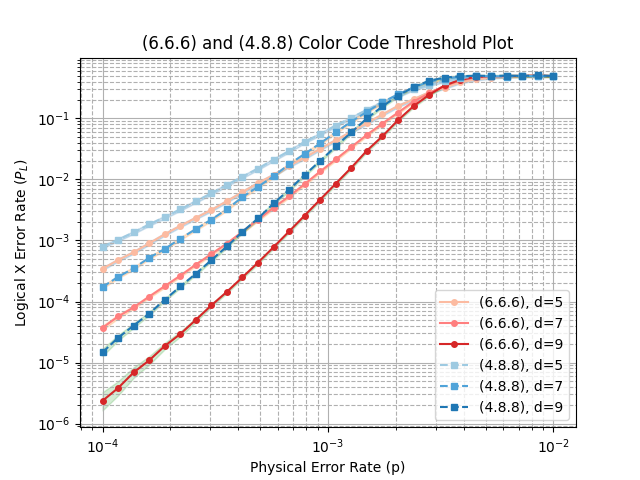
\includegraphics[width=1.2\linewidth]{assets/thresholds/X_Comparison_Threshold_Plot.png}
        \caption{Threshold plot for the logical X error rates}
    \end{subfigure}
    \hfill
    \begin{subfigure}{0.45\textwidth}
        \centering
        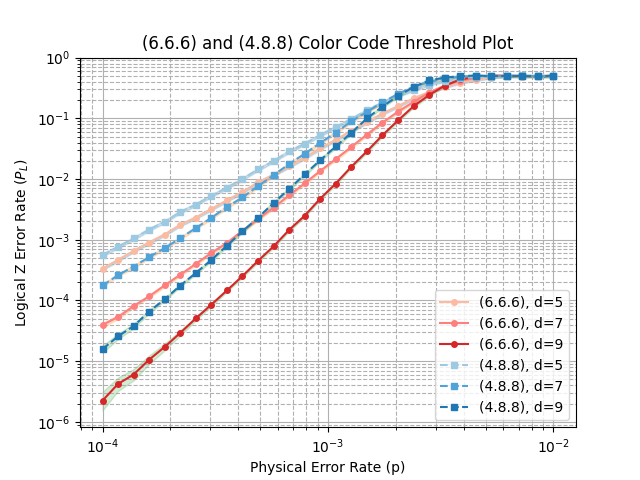
\includegraphics[width=1.2\linewidth]{assets/thresholds/Z_Comparison_Threshold_Plot.png}
        \caption{Threshold plot for the logical Z error rates}
    \end{subfigure}

    \vspace{1em}

    \begin{subfigure}{0.45\textwidth}
        \centering
        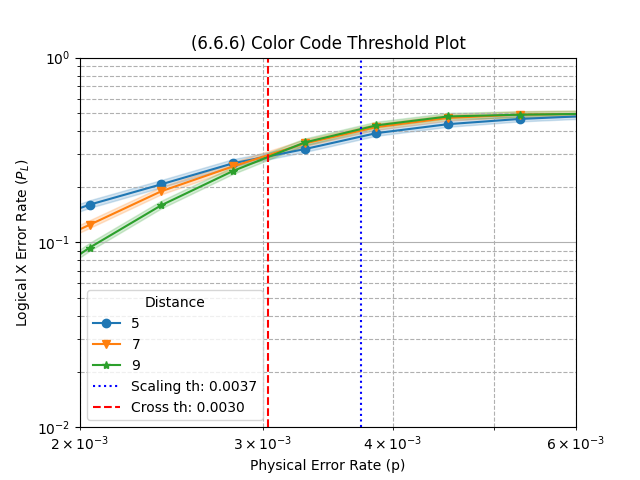
\includegraphics[width=1.2\linewidth]{assets/thresholds/ImplCCThresholdPlot_666_Final_XL_Zoomed.png}
        \caption{Scaling and cross thresholds on (6.6.6) logical X plot}
    \end{subfigure}
    \hfill
    \begin{subfigure}{0.45\textwidth}
        \centering
        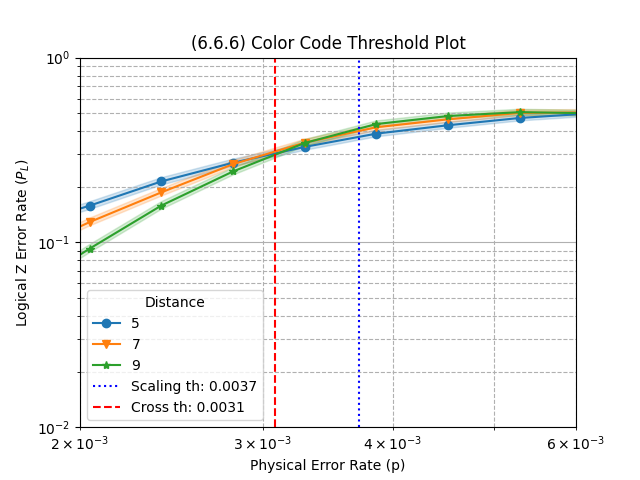
\includegraphics[width=1.2\linewidth]{assets/thresholds/ImplCCThresholdPlot_666_Final_ZL_Zoomed.png}
        \caption{Scaling and cross thresholds on (6.6.6) logical Z plot}
    \end{subfigure}

    \vspace{1em}

    % --- Second row of two images ---
    \begin{subfigure}{0.45\textwidth}
        \centering
        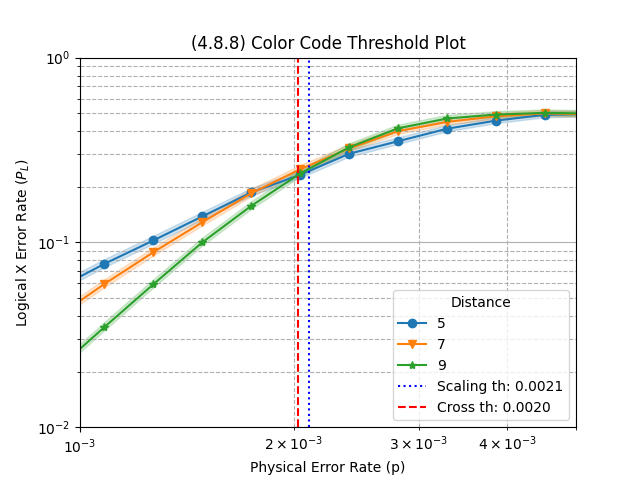
\includegraphics[width=1.2\linewidth]{assets/thresholds/ImplCCThresholdPlot_488_Final_XL_Zoomed.png}
        \caption{Scaling and cross thresholds on (4.8.8) logical X plot}
    \end{subfigure}
    \hfill
    \begin{subfigure}{0.45\textwidth}
        \centering
        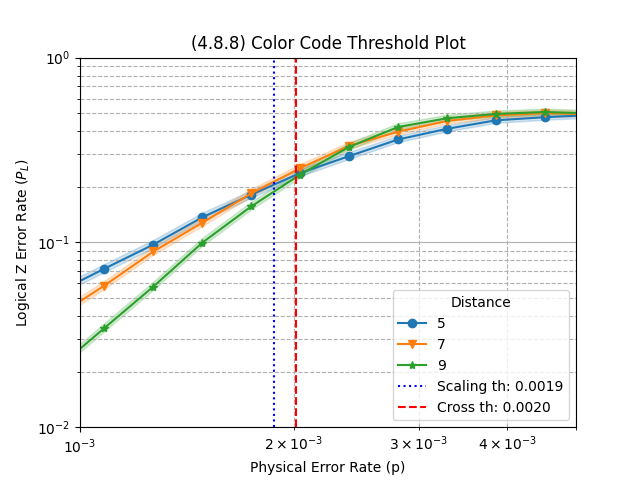
\includegraphics[width=1.2\linewidth]{assets/thresholds/ImplCCThresholdPlot_488_Final_ZL_Zoomed.png}
        \caption{Scaling and cross thresholds on (4.8.8) logical Z plot}
    \end{subfigure}

    \caption{Threshold plots for the (6.6.6) color code implementations, with both thresholds indicated as vertical lines on the lower plots}
    \label{fig:all_plots}
\end{figure}

We achieve thresholds within the expected performance range of $0.2-0.47\%$ for (6.6.6) color codes under circuit level noise. The thresholds for the (4.8.8) color codes also occur between the $0.14(1) - 0.29(1)\%$ ranges achieved in this paper, including the optimised circuits, with our threshold being slightly above the baseline's single-ancilla thresholds.

This performance gap is likely driven by the difference in decoding methodologies. The baseline paper uses an integer programming decoder, using uniform weights for their single-ancilla circuits, implicitly using an independence assumption such that the decoder may fail to account for the impact of correlated errors such as hook errors. In contrast, this project uses chromobius, which can natively resolve these correlated errors. Rather than relying on uniform-weight assumptions, the decoder utilises colour information in the circuits to build connected subgraphs that enable tracing of complex error chains, allowing the detector to identify certain single-qubit faults that propagate into multi-qubit symptoms.

\section{Qubit Mapping}
\label{sec:qubit_mapping_eval}
As established in Section \ref{sec:impl_qubit_mapping}, the physical viability of color codes on QCCD architectures hinges on the efficiency of mapping their topological structures to hardware traps. This section evaluates the operational impact of its three distinct algorithmic variants: \begin{itemize}
    \item Bounded distance merging
    \item Unbounded distance merging
    \item k-nearest-neighbour merging
\end{itemize}

Because each strategy imposes different geometric constraints during the merging phase, they generate fundamentally distinct hardware clusters. These clustering variations directly dictate the required ion routing schedules, thereby impacting the overall compilation overhead and final logical error rates. To assess these impacts, this section comprehensively benchmarks the three merging strategies against the baseline framework's clustering strategy across varying QCCD trap capacities and projected hardware gate fidelities.

%Furthermore, to validate the architectural parameters within the most resource-constrained regimes, this evaluation will also feature a sensitivity analysis exploring the consequences of varying the bounded merging strategy's distance threshold.

Using the (6.6.6) color code circuits developed in Section \ref{sec:impl_color_code}, the circuits ranging in distances from 3 to 9, were compiled onto a grid QCCD architecture over trap capacities ranging from 2 to 120. Additionally, these experiments were performed under different physical error rates, dictated by a \textbf{gate improvement} factor in the simulation. For example, a 5x gate improvement corresponds to 5x lower gate errors, roughly in the order of $10^{-3}$, depicting rates akin to QCCD devices from Quantinuum \cite{quantinuum_performance_validation}.

As established in Section \ref{sec:color_code_eval}, our threshold lies in the order of $10^3$, so we are particularly interested in the behaviour of the schemes around and below these rates, given by gate improvements 5x and 10x.



\subsection{Results}


The logical error rates achieved from these experiments are outlined through a comparative heatmap, coloured by the $\log_{10}$ ratio between the proposed and baseline clustering schemes. Negative values (blue) indicate superior performance of the proposed algorithm for a given code distance and trap capacity.

\begin{figure}[htbp]
    \centering
    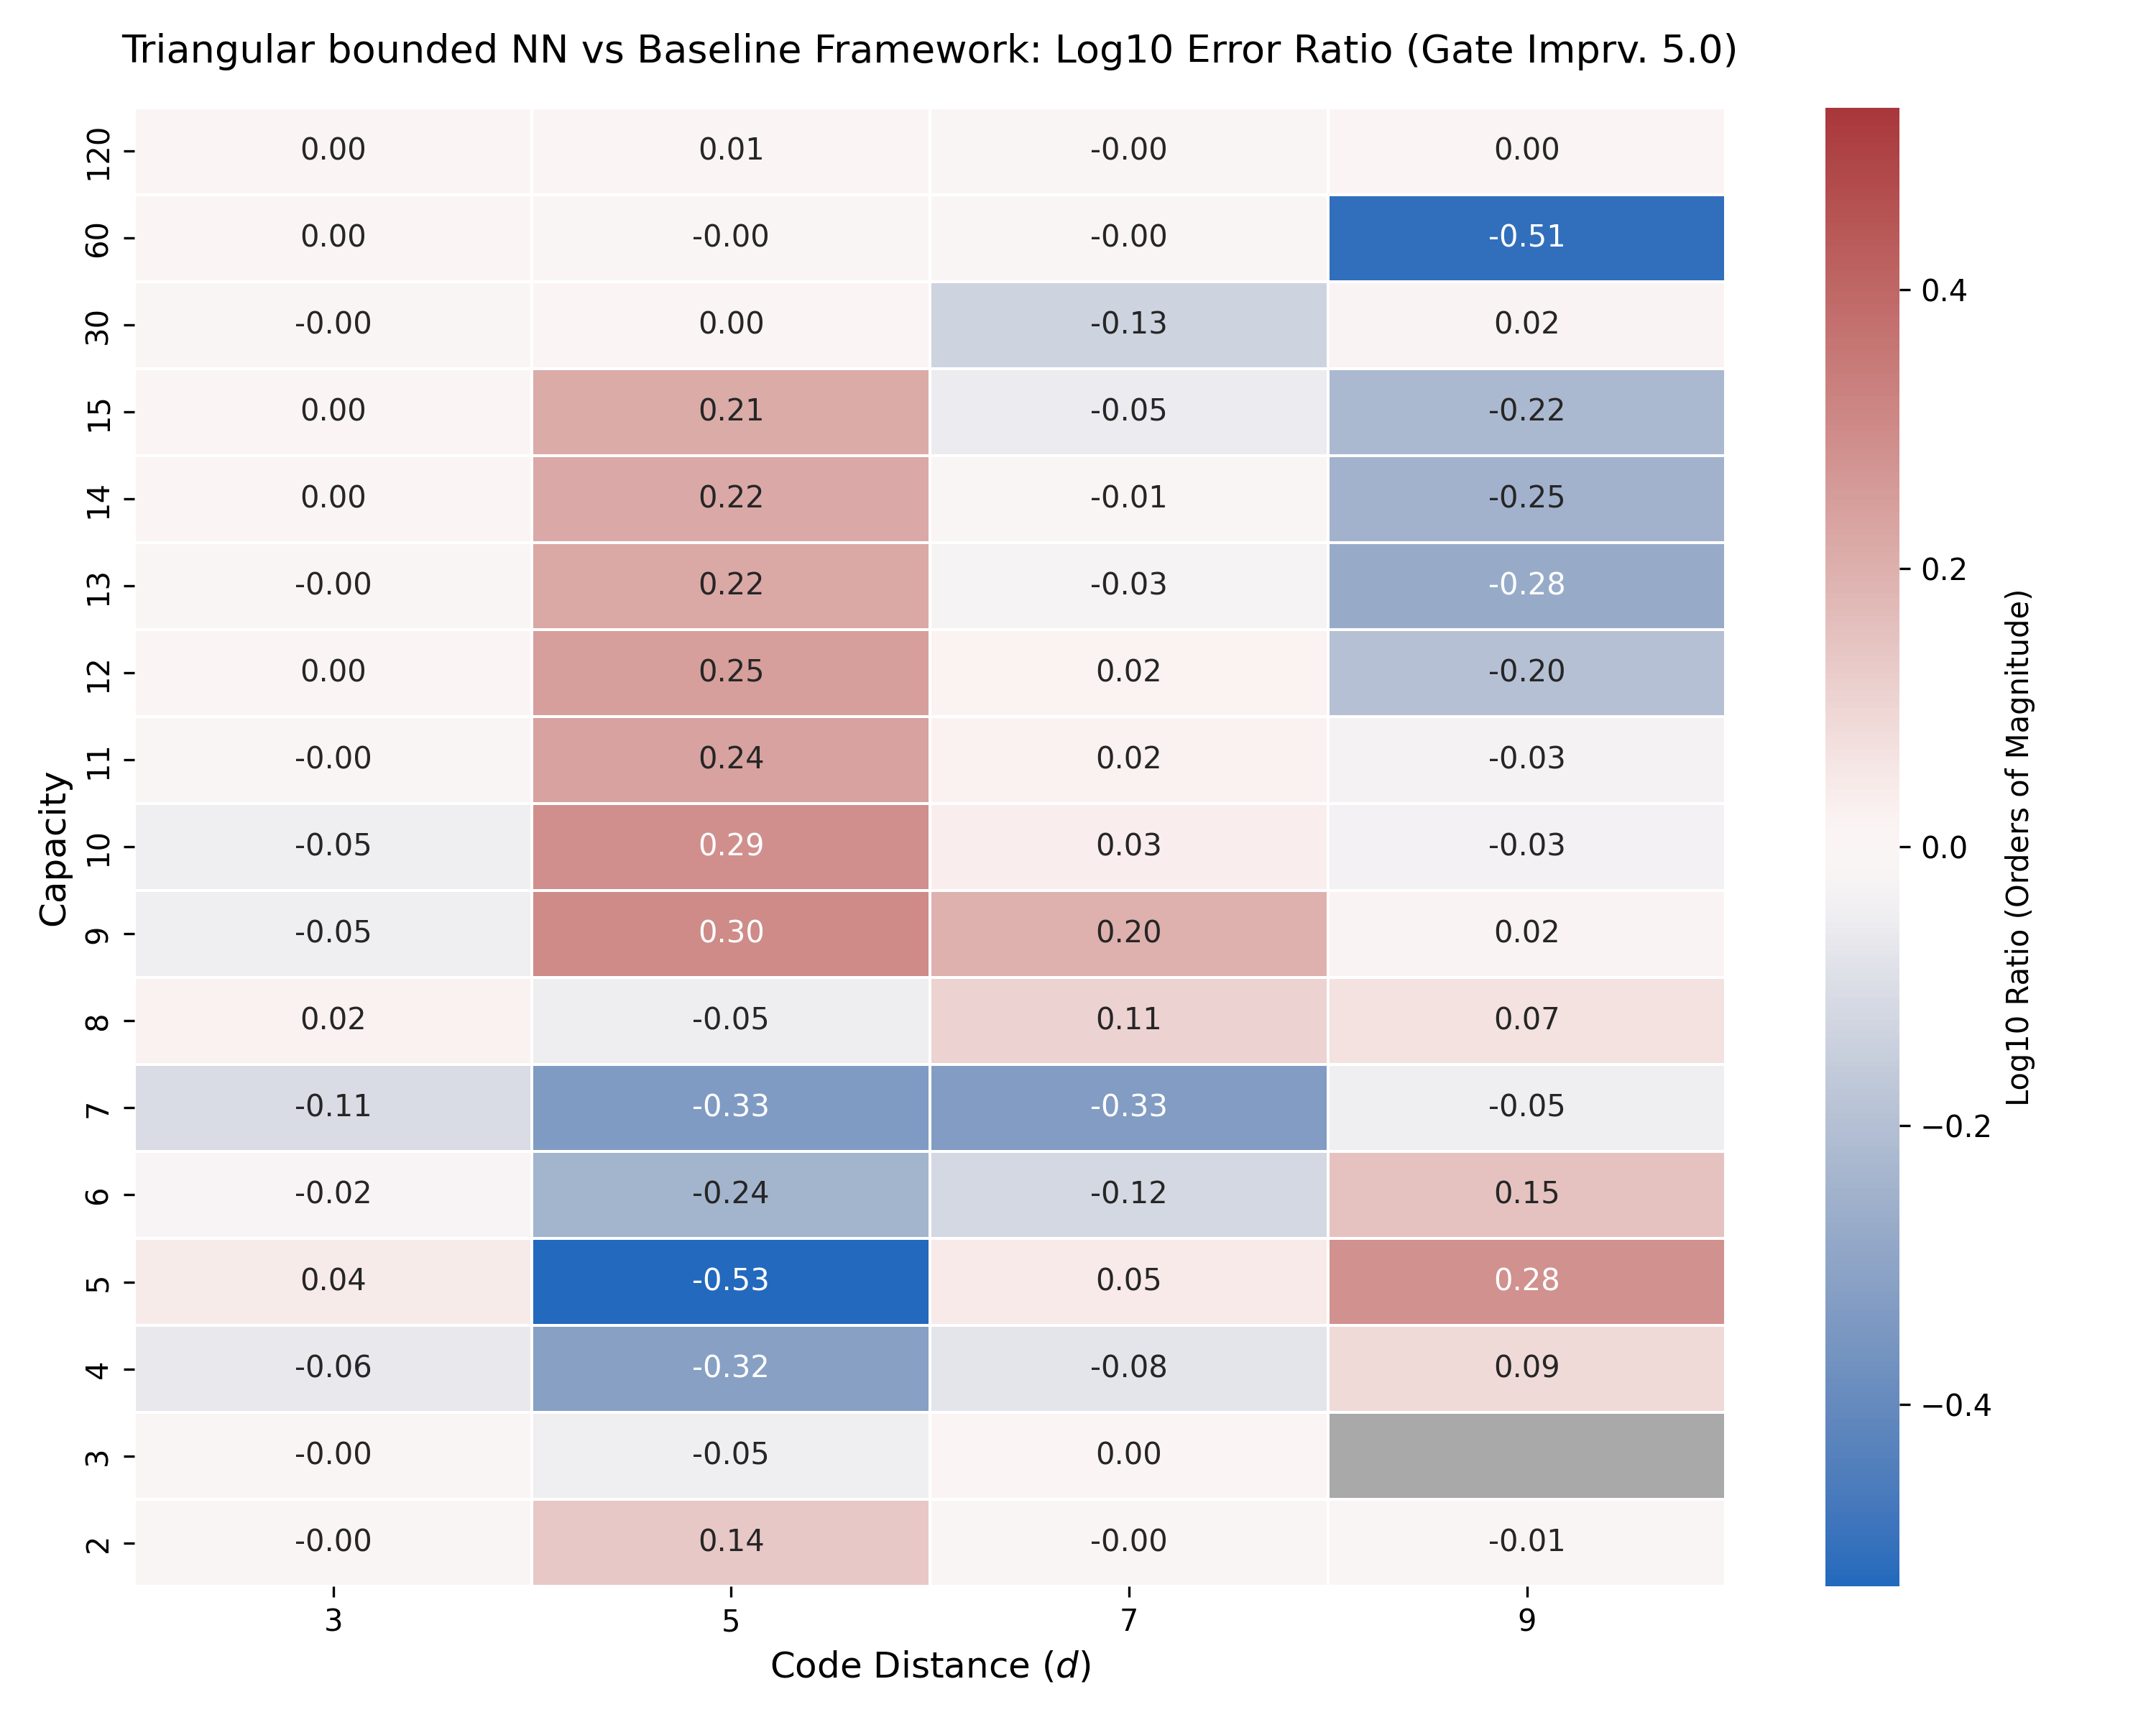
\includegraphics[width=0.75\linewidth]{assets/heatmaps/heatmap_logratio_factor_5.0_Triangular_bounded_NN.png}
    \caption{Benchmark of the logical error rates of the \textbf{bounded distance scheme} against the baseline.}
    \label{fig:boundedheatmap}
\end{figure}

\begin{figure}[htbp]
    \centering
    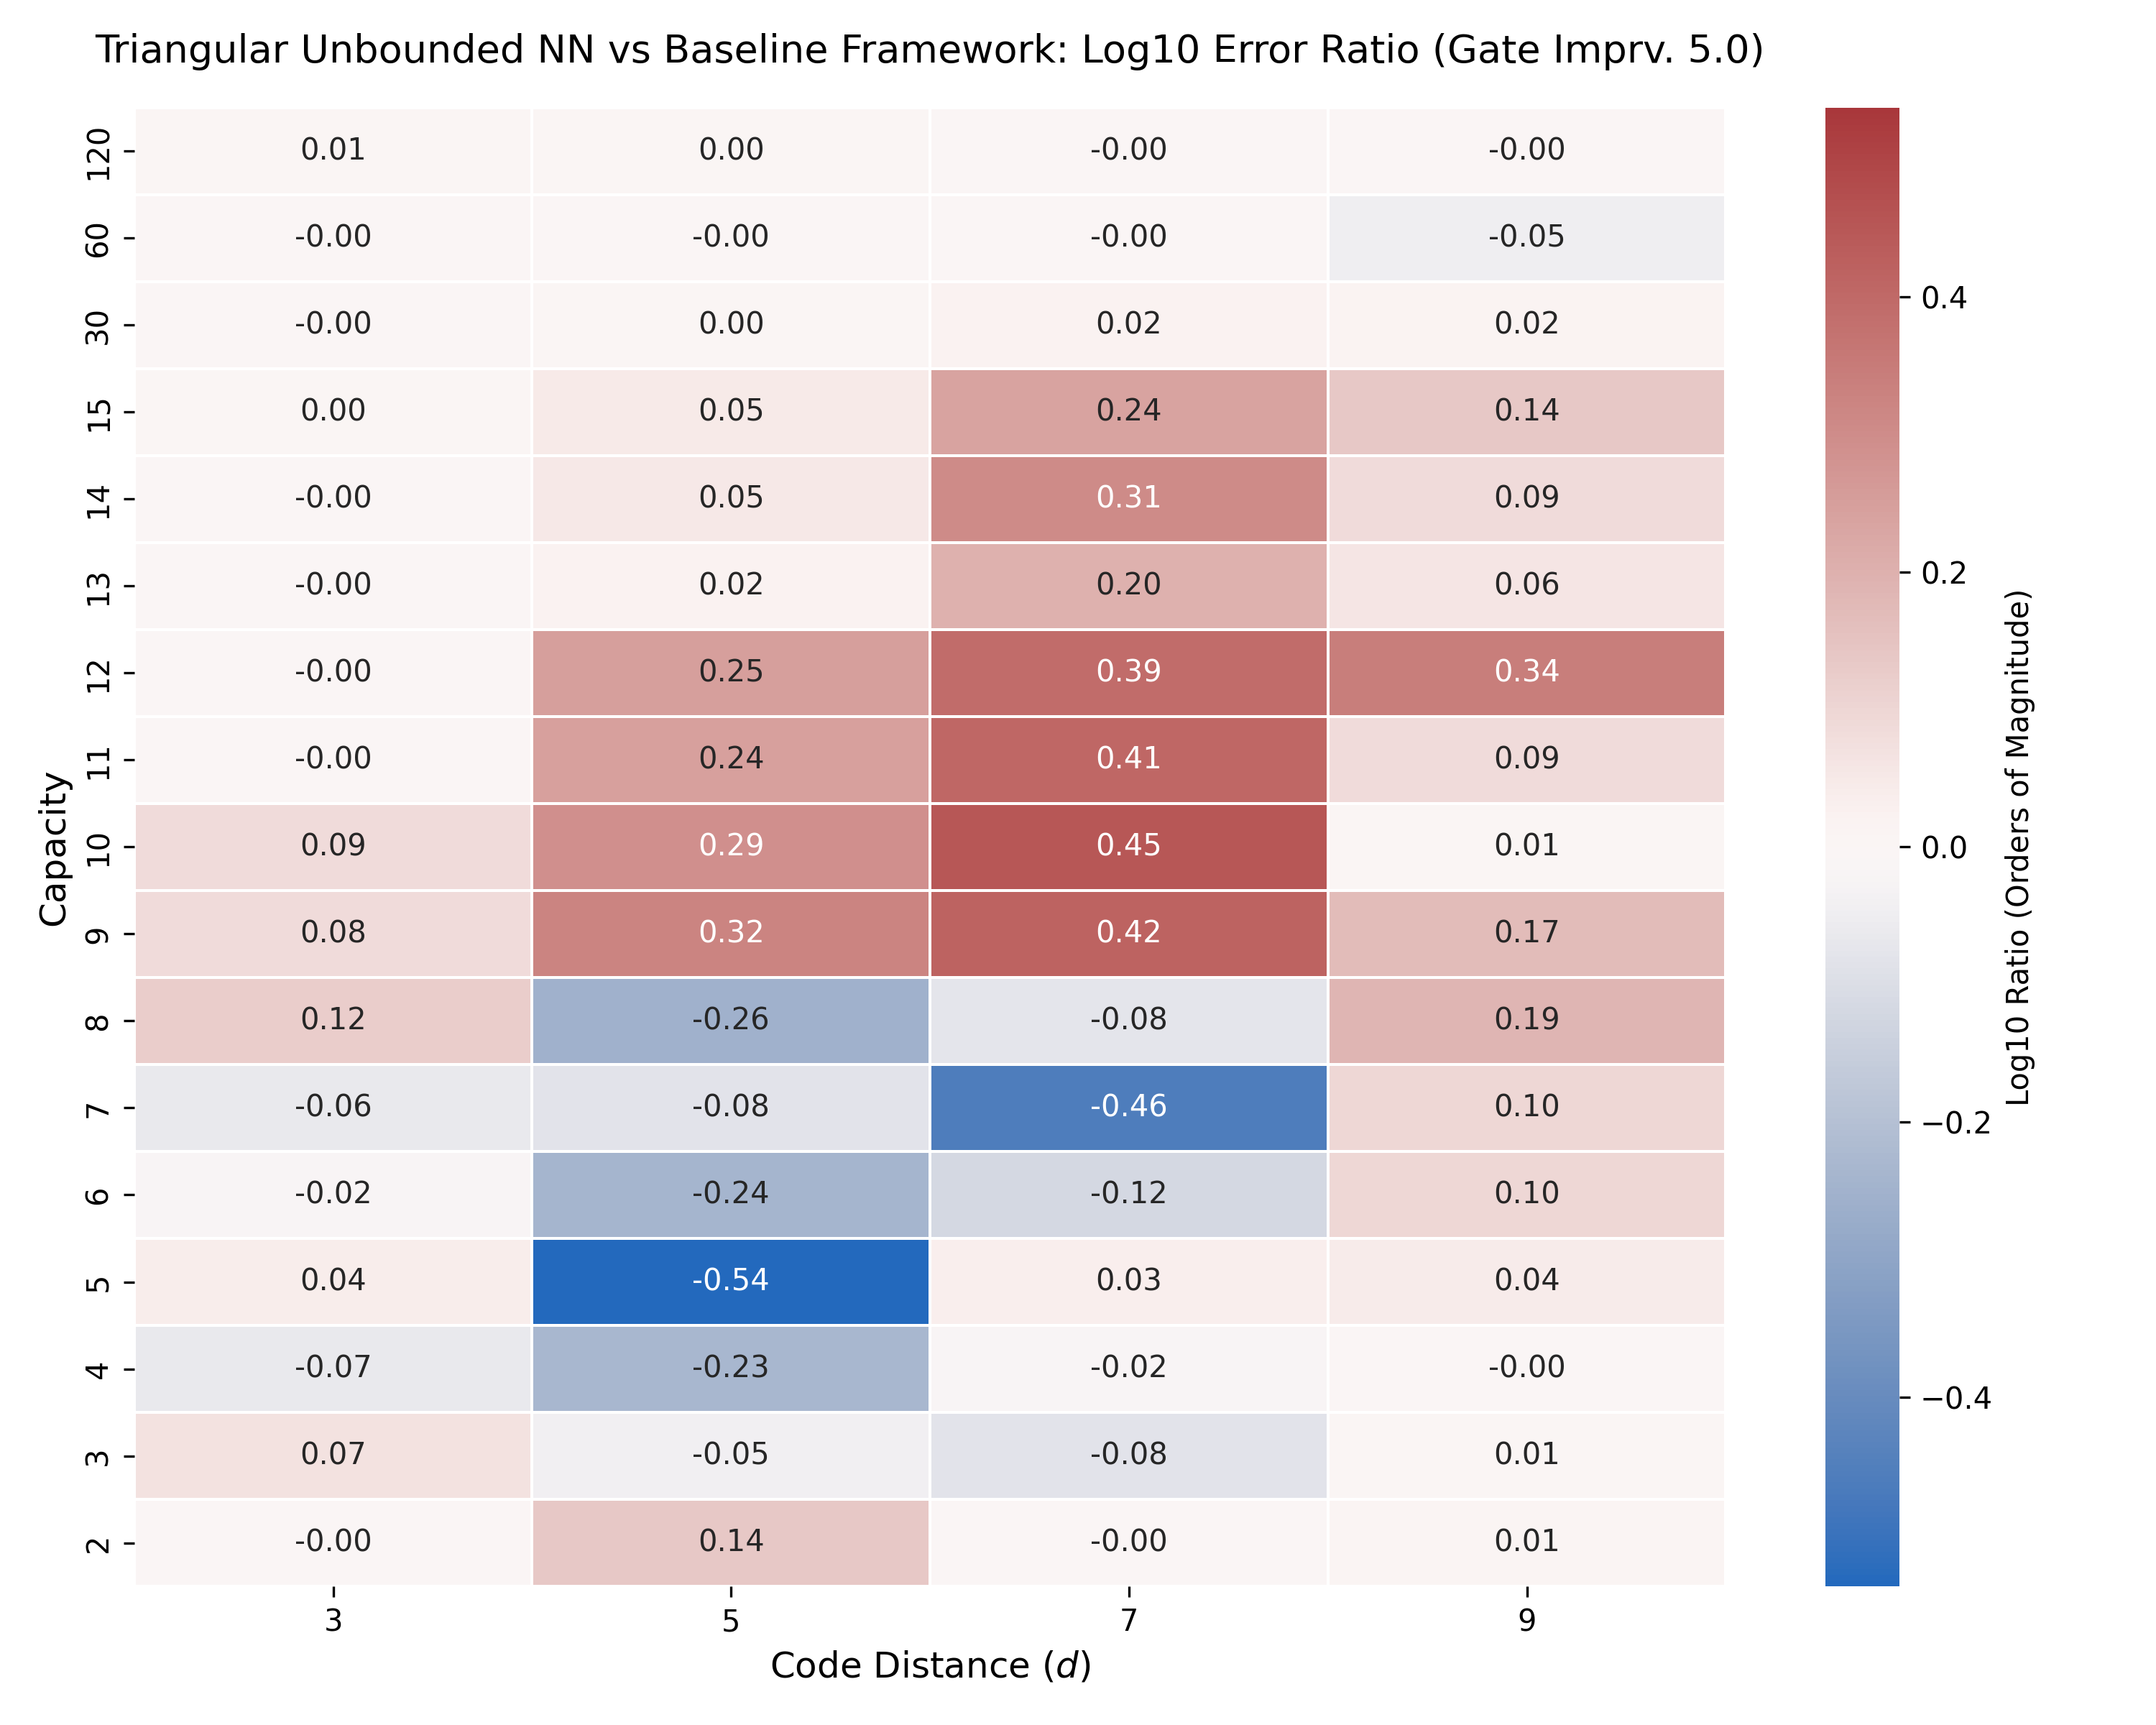
\includegraphics[width=0.75\linewidth]{assets/heatmaps/heatmap_logratio_factor_5.0_Triangular_Unbounded_NN.png}
    \caption{Benchmark of the logical error rates of the \textbf{unbounded distance scheme} against the baseline.}
    \label{fig:unboundedheatmap}
\end{figure}    

\begin{figure}[htbp]
    \centering
    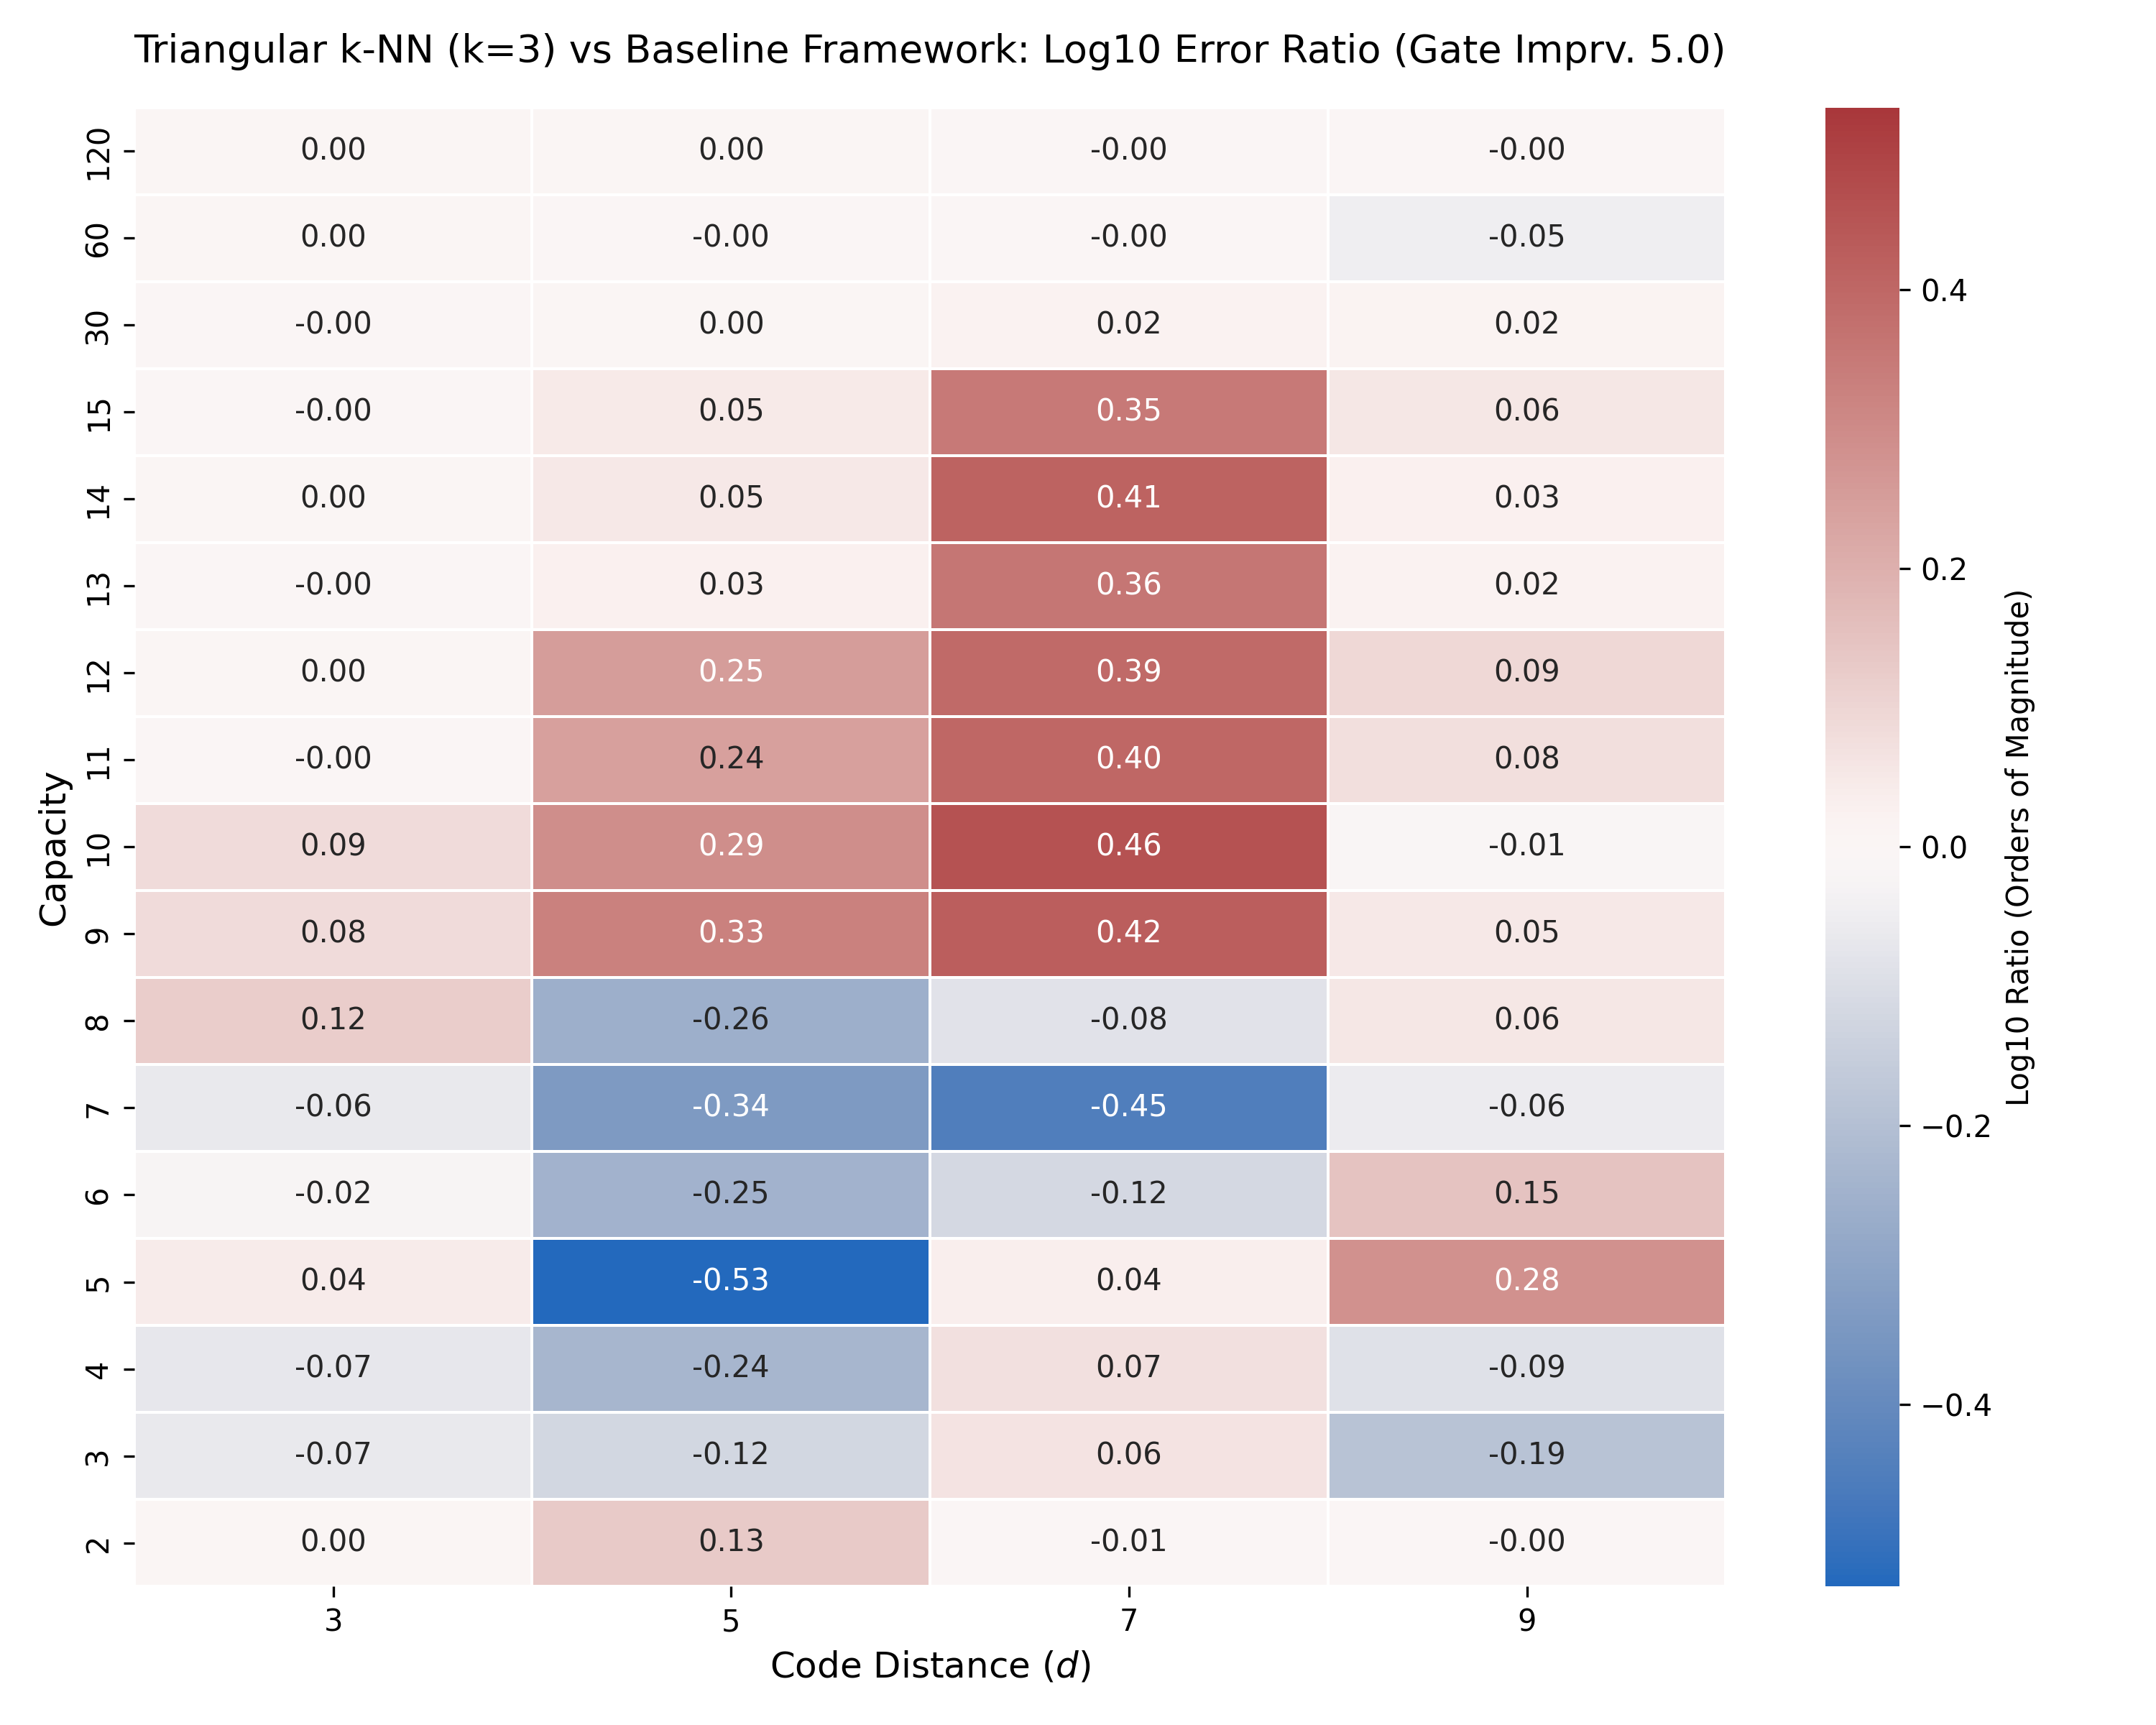
\includegraphics[width=0.75\linewidth]{assets/heatmaps/heatmap_logratio_factor_5.0_Triangular_k-NN_(k=3).png}
    \caption{Benchmark of the logical error rates of the \textbf{k-NN scheme} against the baseline.}
    \label{fig:knnheatmap}
\end{figure}

The most critical insight derived from Fig. \ref{fig:boundedheatmap}, Fig. \ref{fig:unboundedheatmap} and Fig. \ref{fig:knnheatmap}, occurs within the resource-constrained region (trap capacities $C\leq 7$). Here, all three mapping strategies demonstrate significant error suppression capabilities, yielding up to a \textbf{3.47x improvement} over the baseline (e.g. -0.54 at $d=5$, $C=4$). This strongly suggests that strictly enforcing the topological locality of the color code is essential when physical hardware is highly fragmented. In the wider context of near-term QCCD development, where modular traps are strictly capacity-limited, this suggests that topology-aware compilation passes for topological QEC codes are highly significant in achieving lower error rates.

Interestingly, the bounded distance merging methodology also performs well in the high-capacity region for distance 9 codes, particularly around $12\leq C\leq 15$ and $C=60$. Whilst the baseline's greedy mechanism produces clusters maximising trap utilisation, this can ultimately reduce the available parallelism in the routing schedule. The constraints of the bounded strategy produces smaller, geometrically regular sub-regions, which provides a schedule parallelisation advantage and retains high locality within traps. 
This can point to the efficacy of maintaining compact, high locality clusters when mapping larger codes onto larger hardware, rather than a greedy, capacity-maximising mapping scheme.

While the proposed methodologies excel in constrained environments, the baseline framework retains a marginal advantage in the intermediate region where $8\leq C \leq 15$. In this domain, the strict geometric partitioning of our triangular clustering occasionally isolates peripheral data qubits into separate traps and suffers from over-clustering, inflating the inter-trap shuttling overhead. Conversely, the baseline's heuristic acts greedily, grouping these edge qubits efficiently. A trade-off is seen when designing mapping methods onto hardware, where enforcing rigid topological structures offers huge payoffs in small capacity devices, but introduces routing penalties when hardware constraints are slightly relaxed.

Above a certain trap capacity (depending on the code distance), the performances of the proposed and baseline mapping schemes are roughly identical. At this point, the entire logical color code can be mapped into a single or dual-trap configuration, resulting in  negligible routing overhead differences between the algorithms. 

It is clear that complex, topology-aware mapping methodologies are specifically vital for more highly distributed, modular QCCD architectures anticipated in the near future, as established by Kielpinski et al. \cite{qccd2002} and demonstrated in commercial architectures \cite{honeywellqccd, quantinuumH2}, rather than monolithic, high-capacity trap designs that limit scalability \cite{wineland1998experimental, hughes1996decoherence}.




\section{Project Requirements Review}



\section{Project Success Criteria}
